\begin{frame}{Vertival error of $d(K^-, n)"\pi^{\mp}\Sigma^{\pm}"$}
  \small
  \begin{tabular}{cc}
    \begin{minipage}{0.5\hsize}
      \begin{figure}
        \centering
        \footnotesize
        $d(K^-, n)"\pi^{\mp}\Sigma^{\pm}"$
        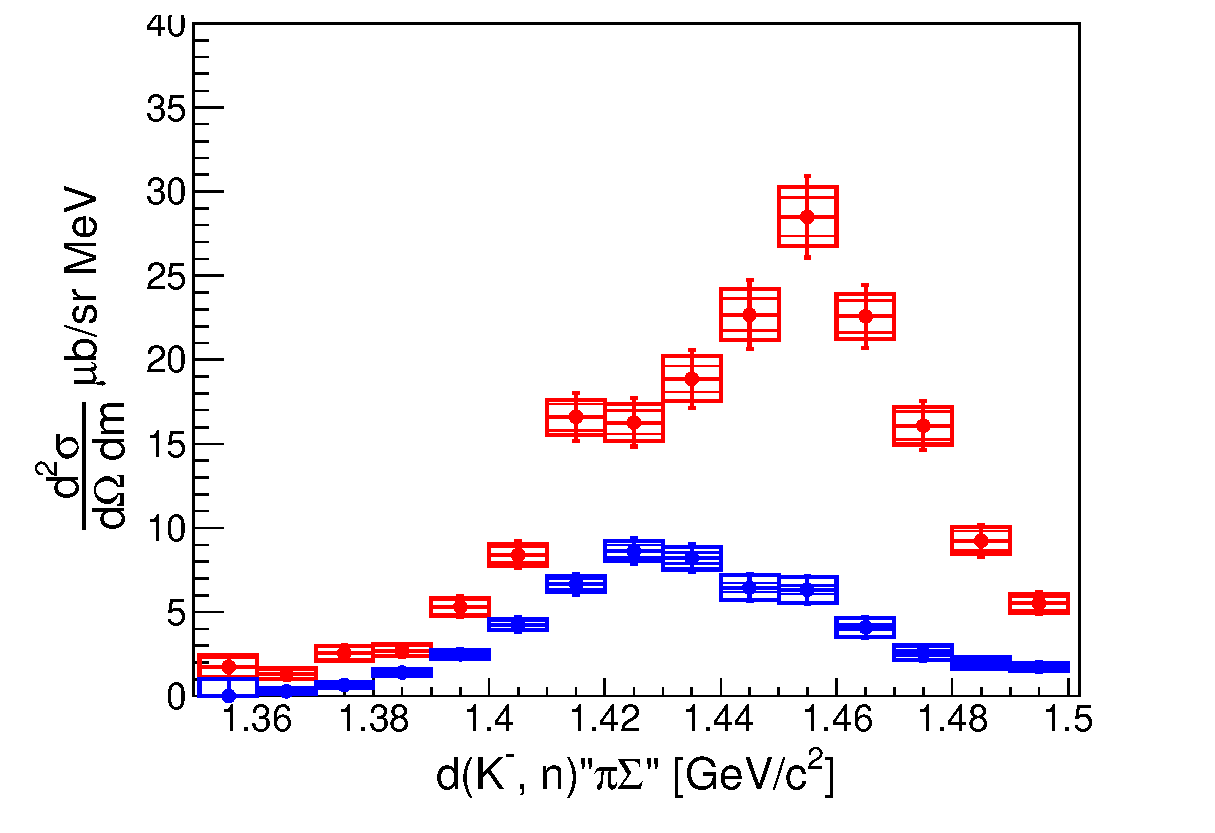
\includegraphics[width=4cm]{../pic/Run78/K0_ts_L1520/ChargeCS_after.eps}
      \end{figure}
    \end{minipage}
    \begin{minipage}{0.5\hsize}
      \begin{figure}
        \centering
        \footnotesize
        Average CS\\
        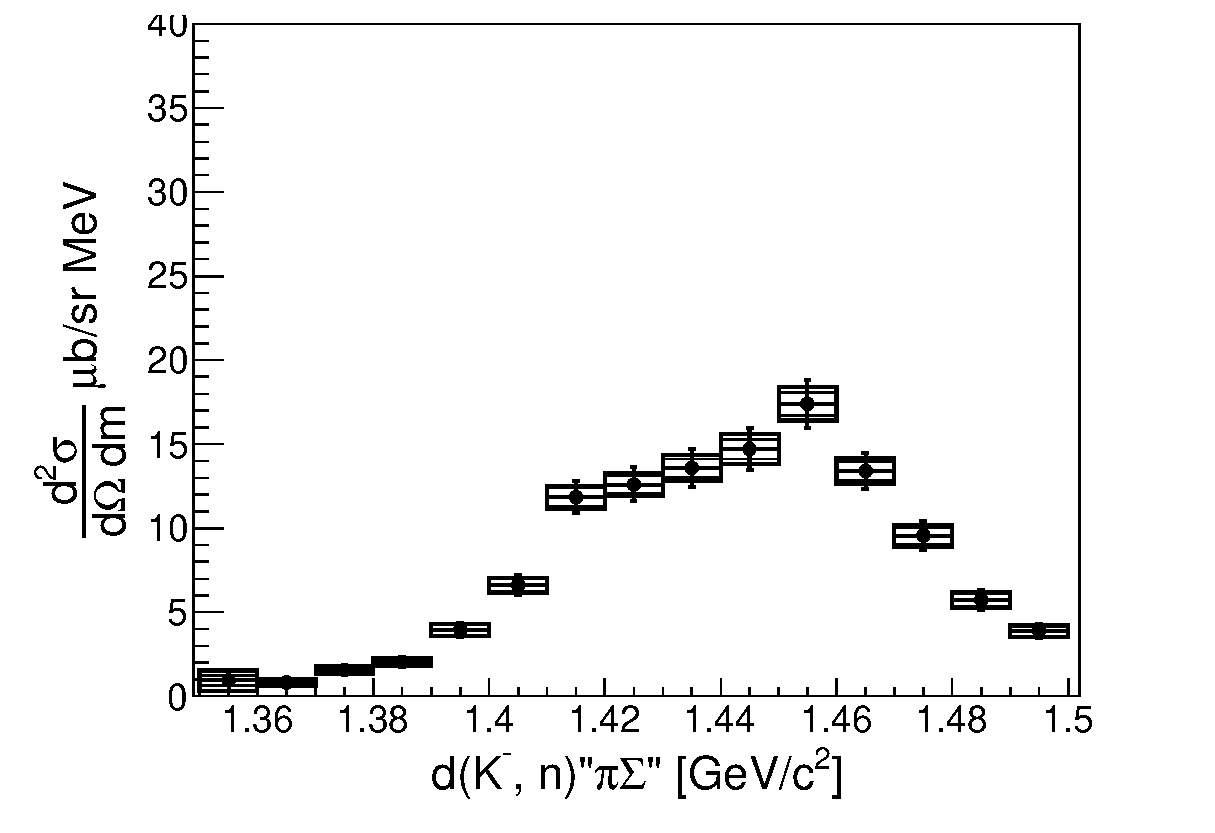
\includegraphics[width=4cm]{../pic/Run78/K0_ts_L1520/ChargeCS_ave_after.eps}
      \end{figure}
    \end{minipage}
  \end{tabular}
  \centering
  \footnotesize
  Inner (thin line) box represents staticial error of $d(K^-, n \pi^+ \pi^-)"n"$ events.\\
  Outer (thick line) box represents errors including template fitting ($d(K^-, n \pi^{\mp})"\Sigma^{\pm}"$).\\
  These two errors are different in each bins.\\
  error bar represents errors added convert factor which is common factor in each bins.
  These errors was convolved as RMS.
  \vspace{3mm}\\
  \small
  for one's information
  \vspace{1.5mm}\\
  Representative value of all errors each spectra\\
%%  Systematic error of template fitting ($d(K^-, n \pi^{\mp})"\Sigma^{\pm}"$) against maximum value\\
  $\rightarrow$ $d(K^-, n \pi^-)"\Sigma^+" \sim 8.6\%$ $d(K^-, n \pi^+)"\Sigma^-" \sim 10.0\%$ average$\sim 8.1\%$


\end{frame}
